%!TEX program = pdflatex
\documentclass{standalone}
\usepackage[UTF8]{ctex}
\usepackage{caption}
\usepackage{amsmath}
\usepackage{tikz}
\usepackage{mathdots}
\usepackage{yhmath}
\usepackage{cancel}
\usepackage{color}
\usepackage{siunitx}
\usepackage{array}
\usepackage{multirow}
\usepackage{amssymb}
\usepackage{gensymb}
\usepackage{tabularx}
\usepackage{booktabs}
\usetikzlibrary{fadings}
\tikzset{every picture/.style={line width=0.75pt}} %set default line width to 0.75pt    

\begin{document}



\tikzset{every picture/.style={line width=0.75pt}} %set default line width to 0.75pt        

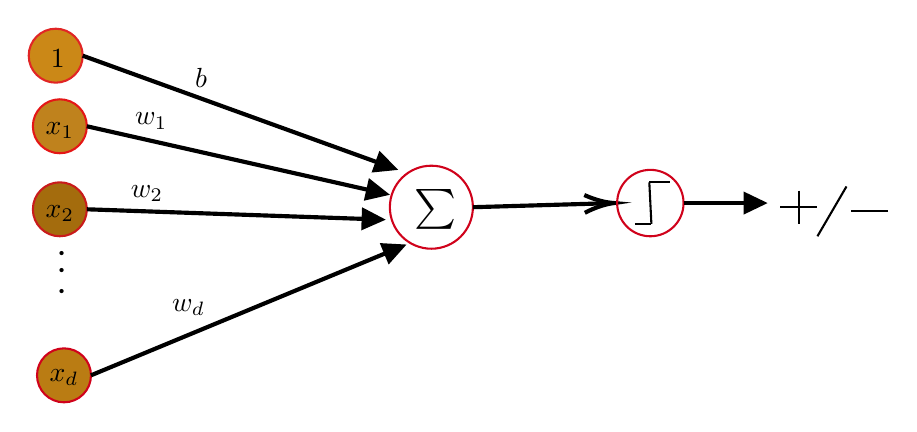
\begin{tikzpicture}[x=0.75pt,y=0.75pt,yscale=-1,xscale=1]
%uncomment if require: \path (0,635.1999969482422); %set diagram left start at 0, and has height of 635.1999969482422

%Shape: Circle [id:dp0181266606691447] 
\draw  [color={rgb, 255:red, 225; green, 37; blue, 37 }  ,draw opacity=1 ][fill={rgb, 255:red, 203; green, 136; blue, 23 }  ,fill opacity=1 ] (164,77) .. controls (164,69.82) and (169.82,64) .. (177,64) .. controls (184.18,64) and (190,69.82) .. (190,77) .. controls (190,84.18) and (184.18,90) .. (177,90) .. controls (169.82,90) and (164,84.18) .. (164,77) -- cycle ;
%Shape: Circle [id:dp20233014296115925] 
\draw  [color={rgb, 255:red, 228; green, 22; blue, 22 }  ,draw opacity=1 ][fill={rgb, 255:red, 191; green, 130; blue, 29 }  ,fill opacity=1 ] (166,111) .. controls (166,103.82) and (171.82,98) .. (179,98) .. controls (186.18,98) and (192,103.82) .. (192,111) .. controls (192,118.18) and (186.18,124) .. (179,124) .. controls (171.82,124) and (166,118.18) .. (166,111) -- cycle ;
%Shape: Circle [id:dp8218852914313741] 
\draw  [color={rgb, 255:red, 208; green, 2; blue, 27 }  ,draw opacity=1 ][fill={rgb, 255:red, 186; green, 124; blue, 19 }  ,fill opacity=1 ] (168,231) .. controls (168,223.82) and (173.82,218) .. (181,218) .. controls (188.18,218) and (194,223.82) .. (194,231) .. controls (194,238.18) and (188.18,244) .. (181,244) .. controls (173.82,244) and (168,238.18) .. (168,231) -- cycle ;
%Shape: Circle [id:dp8974374066301434] 
\draw  [color={rgb, 255:red, 201; green, 27; blue, 27 }  ,draw opacity=1 ][fill={rgb, 255:red, 164; green, 108; blue, 13 }  ,fill opacity=1 ] (166,151) .. controls (166,143.82) and (171.82,138) .. (179,138) .. controls (186.18,138) and (192,143.82) .. (192,151) .. controls (192,158.18) and (186.18,164) .. (179,164) .. controls (171.82,164) and (166,158.18) .. (166,151) -- cycle ;
%Shape: Circle [id:dp8670311761560525] 
\draw  [color={rgb, 255:red, 208; green, 2; blue, 27 }  ,draw opacity=1 ] (338,150) .. controls (338,138.95) and (346.95,130) .. (358,130) .. controls (369.05,130) and (378,138.95) .. (378,150) .. controls (378,161.05) and (369.05,170) .. (358,170) .. controls (346.95,170) and (338,161.05) .. (338,150) -- cycle ;
%Straight Lines [id:da5539890140009067] 
\draw [line width=1.5]    (190,77) -- (339.18,130.98) ;
\draw [shift={(342,132)}, rotate = 199.89] [fill={rgb, 255:red, 0; green, 0; blue, 0 }  ][line width=1.5]  [draw opacity=0] (11.61,-5.58) -- (0,0) -- (11.61,5.58) -- cycle    ;

%Straight Lines [id:da9150166432056007] 
\draw [line width=1.5]    (192,111) -- (335.07,143.34) ;
\draw [shift={(338,144)}, rotate = 192.74] [fill={rgb, 255:red, 0; green, 0; blue, 0 }  ][line width=1.5]  [draw opacity=0] (11.61,-5.58) -- (0,0) -- (11.61,5.58) -- cycle    ;

%Straight Lines [id:da21785183094429172] 
\draw [line width=1.5]    (192,151) -- (333,155.9) ;
\draw [shift={(336,156)}, rotate = 181.99] [fill={rgb, 255:red, 0; green, 0; blue, 0 }  ][line width=1.5]  [draw opacity=0] (11.61,-5.58) -- (0,0) -- (11.61,5.58) -- cycle    ;

%Straight Lines [id:da07631841782076165] 
\draw [line width=1.5]    (194,231) -- (343.23,169.15) ;
\draw [shift={(346,168)}, rotate = 517.49] [fill={rgb, 255:red, 0; green, 0; blue, 0 }  ][line width=1.5]  [draw opacity=0] (11.61,-5.58) -- (0,0) -- (11.61,5.58) -- cycle    ;

%Straight Lines [id:da09258077968651568] 
\draw [line width=1.5]    (378,150) -- (443,148.09) ;
\draw [shift={(446,148)}, rotate = 538.3199999999999] [color={rgb, 255:red, 0; green, 0; blue, 0 }  ][line width=1.5]    (14.21,-4.28) .. controls (9.04,-1.82) and (4.3,-0.39) .. (0,0) .. controls (4.3,0.39) and (9.04,1.82) .. (14.21,4.28)   ;

%Shape: Circle [id:dp2823819763429941] 
\draw  [color={rgb, 255:red, 208; green, 2; blue, 27 }  ,draw opacity=1 ] (447.5,148) .. controls (447.5,139.16) and (454.66,132) .. (463.5,132) .. controls (472.34,132) and (479.5,139.16) .. (479.5,148) .. controls (479.5,156.84) and (472.34,164) .. (463.5,164) .. controls (454.66,164) and (447.5,156.84) .. (447.5,148) -- cycle ;
%Straight Lines [id:da946632337518059] 
\draw    (463,138) -- (473,138) ;


%Straight Lines [id:da3679992777592641] 
\draw    (464,158) -- (463,138) ;


%Straight Lines [id:da10911669037887384] 
\draw    (456,158) -- (464,158) ;


%Straight Lines [id:da1323721896884582] 
\draw [line width=1.5]    (479.5,148) -- (517,148) ;
\draw [shift={(520,148)}, rotate = 180] [fill={rgb, 255:red, 0; green, 0; blue, 0 }  ][line width=1.5]  [draw opacity=0] (11.61,-5.58) -- (0,0) -- (11.61,5.58) -- cycle    ;

\draw   (526,150) -- (544,150)(535,142) -- (535,158) ;
%Straight Lines [id:da4574374069370577] 
\draw    (558,140) -- (544,164) ;


%Straight Lines [id:da561484761447654] 
\draw    (578,152) -- (560,152) ;



% Text Node
\draw (180,181) node [scale=1.44]  {$\cdotp $};
% Text Node
\draw (180,173) node [scale=1.44]  {$\cdotp $};
% Text Node
\draw (180,191) node [scale=1.44]  {$\cdotp $};
% Text Node
\draw (178,78.5) node   {$1$};
% Text Node
\draw (179,113) node   {$x_{1}$};
% Text Node
\draw (179,153) node   {$x_{2}$};
% Text Node
\draw (181,232) node   {$x_{d}$};
% Text Node
\draw (360,151) node [scale=1.44]  {$\sum $};
% Text Node
\draw (247,87.5) node   {$b$};
% Text Node
\draw (223,108.5) node   {$w_{1}$};
% Text Node
\draw (221,143.5) node   {$w_{2}$};
% Text Node
\draw (241,198.5) node   {$w_{d}$};


\end{tikzpicture}

\end{document}
